\section{Discussion}
\label{sec:discussion}

The transition from component-centric vulnerability scanning to compositional attack path scoring represents a fundamental paradigm shift in AI security. Our empirical results validate the core hypothesis of the CAPS framework: securing modern LLM stacks requires continuous, holistic topological analysis. In this section, we discuss the broader theoretical implications of our findings, operational deployment strategies, and inherent limitations.

\subsection{Theoretical Implications of Multi-Hop Friction}
The inclusion of the exponential chaining decay factor ($\alpha$) is not merely a mathematical heuristic; it models a well-documented phenomenon in offensive security. Each transition across an architectural boundary---such as an orchestrator invoking an external API or a prompt gateway querying a vector database---imposes strict constraints on payload delivery. 

\begin{figure}[ht]
    \centering
    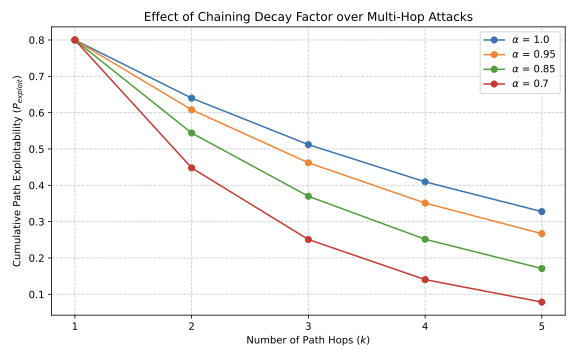
\includegraphics[width=0.8\linewidth]{figures/decay_effect.png}
    \caption{The impact of the chaining decay factor ($\alpha$) on cumulative path exploitability over multiple hops. As path length increases, lower $\alpha$ values correctly penalize the theoretical probability to reflect real-world exploit friction.}
    \label{fig:decay}
\end{figure}

As illustrated in Figure \ref{fig:decay}, the impact of $\alpha$ becomes exponentially pronounced as path length ($k$) increases. While baseline models lacking decay (effectively $\alpha = 1.0$) project a linear or mildly attenuated reduction in exploitability, lower $\alpha$ values drastically restrict the viability of long attack chains. An attacker attempting a 5-hop exploit in a system with $\alpha = 0.85$ faces an inherent theoretical friction penalty that reduces the probability of end-to-end success by over 47\%, even before accounting for component-specific mitigations. This highlights why "assume breach" architectures, which intentionally increase the graph diameter between entry points and critical assets, are highly effective defense strategies.

\subsection{Operational Integration via CI/CD pipelines}
To realize the full value of the CAPS framework, organizations must transition from static, point-in-time risk assessments to continuous evaluation. We propose that the CAPS engine be integrated directly into Continuous Integration and Continuous Deployment (CI/CD) pipelines. 

By defining the deployment architecture as code (e.g., via Terraform or standard JSON topologies), the CAPS engine can be executed automatically on every pull request. If a developer introduces a new tool (creating a new edge in the graph) or downgrades a mitigation, CAPS will instantly recalculate the maximal path score. If the new topology violates a pre-defined risk threshold (e.g., $S_{max} > 50$), the build can be automatically failed. This operationalizes "Security by Design" in LLM ecosystems, providing immediate, quantitative feedback to engineering teams before compositional vulnerabilities reach production environments.

\subsection{Limitations and Future Work}
While CAPS provides a robust structural and mathematical foundation, the accuracy of its outputs is inherently bounded by the fidelity of its inputs. The model currently relies on heuristic or expert-consensus estimations for Base Exploitability ($E$) and Mitigation Effectiveness ($M$). In rapidly evolving fields like Adversarial Machine Learning, these values can fluctuate wildly based on the discovery of novel jailbreak techniques or prompt injection variants.

Future work will focus on dynamic parameter estimation. By integrating automated LLM red-teaming frameworks (such as Promptfoo or Garak) with the CAPS engine, we can continuously bombard components with synthetic payloads. The empirical success rates of these localized attacks can then be fed back into the CAPS graph, enabling dynamic, real-time recalculation of $E(vuln)$ and $M(mit)$. This will effectively close the loop between theoretical risk modeling and empirical validation, yielding a self-tuning, continuous threat assessment ecosystem.
